\subsection{IFIT Subcellular Localisation During Interferon Induction and RSV Infection} \label{subsec:IFIT Subcellular Localisation During Interferon INduction and RSV Infection}
put antibody validation wbs

compare and contrast to the info in databases and papers

% introduction to ib stuff from my study
write about ib size statistics from my analysis


\begin{figure}
    \centering
    \includegraphics[width=1\linewidth]{09. Chapter 4/Figs/01. Localisation introduction/01. IB-zooms.pdf}
    \caption[Representative Infection Zoom.]{\textbf{Representative Infection Zoom.} asdf asdf asdf asdf asdf asdf sdfgsdfg}
    \label{fig:Representative Infection Zoom}
\end{figure}

\begin{figure}
    \centering
    \includegraphics[width=1\linewidth]{09. Chapter 4/Figs/01. Localisation introduction/02. placeholder - ib statistics.png}
    \caption[IB area and diameter per cell line.]{\textbf{IB area and diameter per cell line.} asdf asdf asdf asdf asdf asdf sdfgsdfg}
    \label{fig:IB area and diameter per cell line}
\end{figure}



% human stuff
Asdfasfsdfasdf \newline
IF Mock | INF | Infection \newline
A549 BEAS2B

Merge pictures of clusters of cells looking at changes between subcellular localisation and a clear increase in mean intensity. Graphs show mean intensity changes from all cells imaged.

\begin{figure}
    \centering
    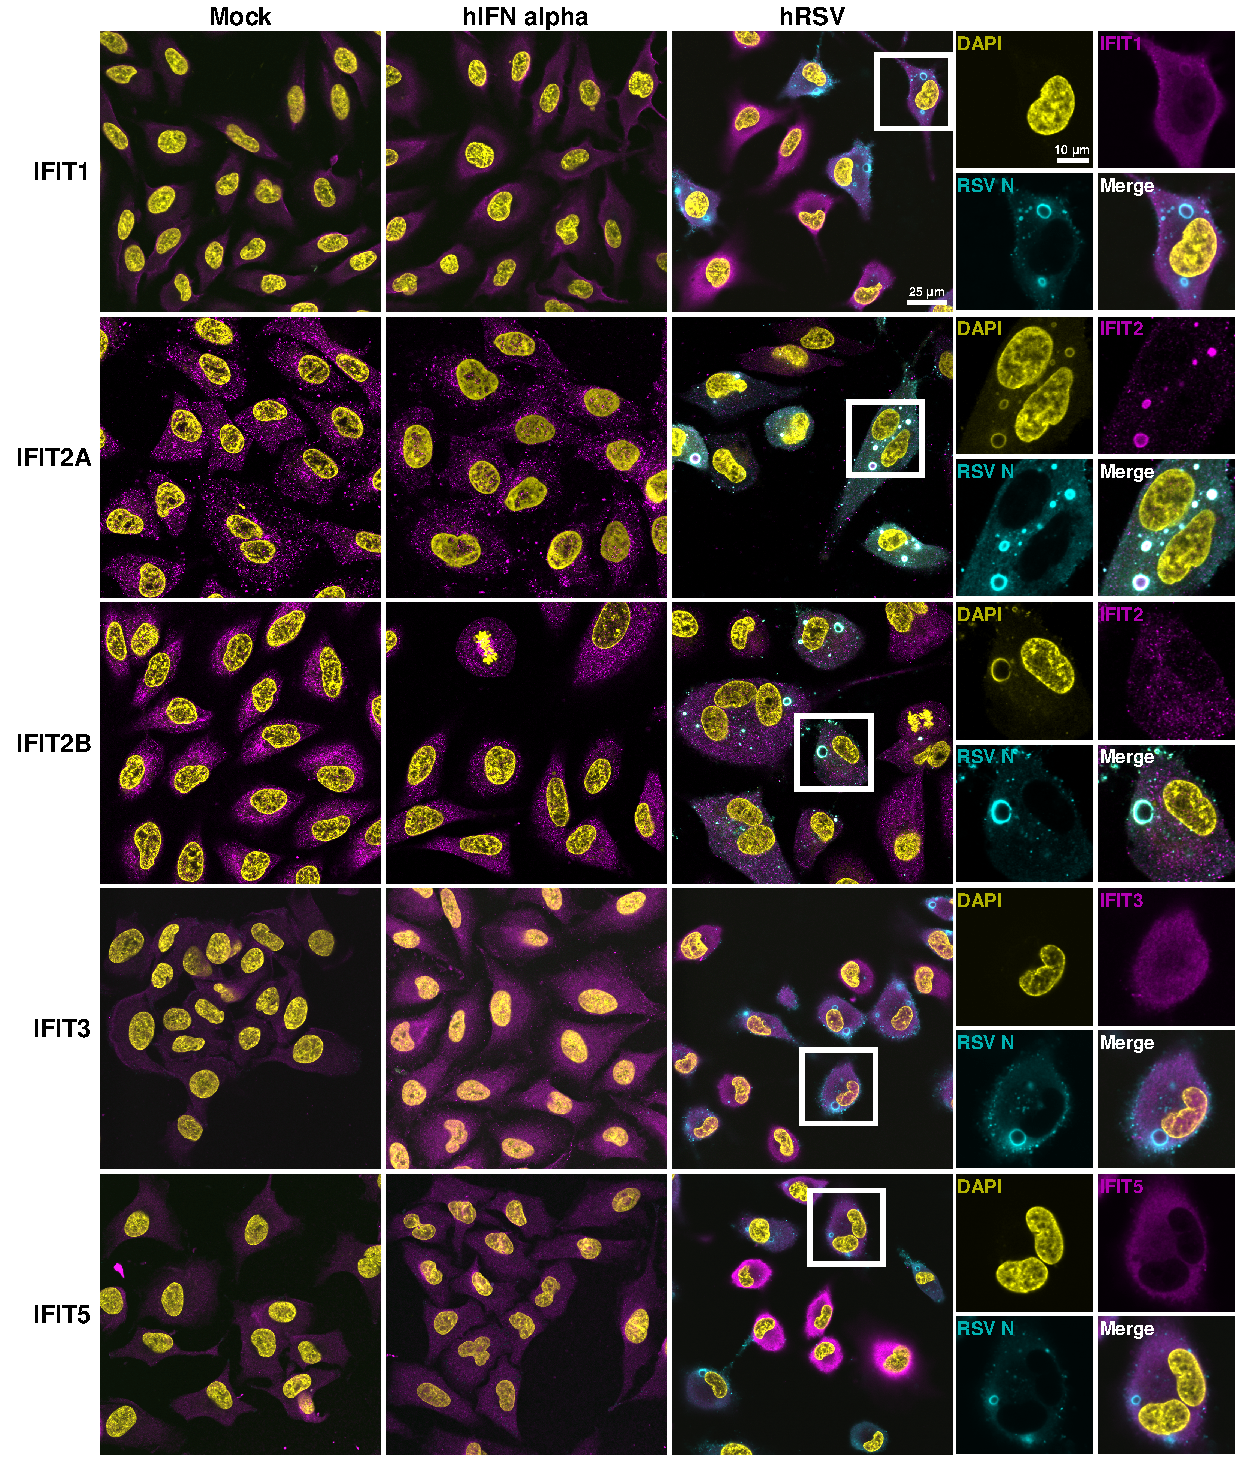
\includegraphics[width=1\linewidth]{09. Chapter 4/Figs/01. Localisation introduction/03. a549 merges.pdf}
    \caption[A549 localisation mergers.]{A549 localisation mergers.}
    \label{fig:A549 localisation mergers.}
\end{figure}


\begin{figure}
    \centering
    \includegraphics[width=1\linewidth]{09. Chapter 4/Figs/01. Localisation introduction/04. a549 plots.png}
    \caption[A549 localisation plots.]{A549 localisation plots.}
    \label{fig:A549 localisation plots.}
\end{figure}


\begin{figure}
    \centering
    \includegraphics[width=0.7\linewidth]{09. Chapter 4/Figs/01. Localisation introduction/05. beas2b merges.png}
    \caption[BEAS2B localisation mergers.]{BEAS2B localisation mergers.}
    \label{fig:BEAS2B localisation mergers.}
\end{figure}


\begin{figure}
    \centering
    \includegraphics[width=1\linewidth]{09. Chapter 4/Figs/01. Localisation introduction/06. beas2b plots.png}
    \caption[BEAS2B localisation plots.]{BEAS2B localisation plots.}
    \label{fig:BEAS2B localisation plots.}
\end{figure}



% bovine stuff
Asdfasfsdfasdf \newline
IF Mock | INF | Infection \newline
MDBK BT

Merge pictures of clusters of cells looking at changes between subcellular localisation and a clear increase in mean intensity. Graphs show mean intensity changes from all cells imaged.

\begin{figure}
    \centering
    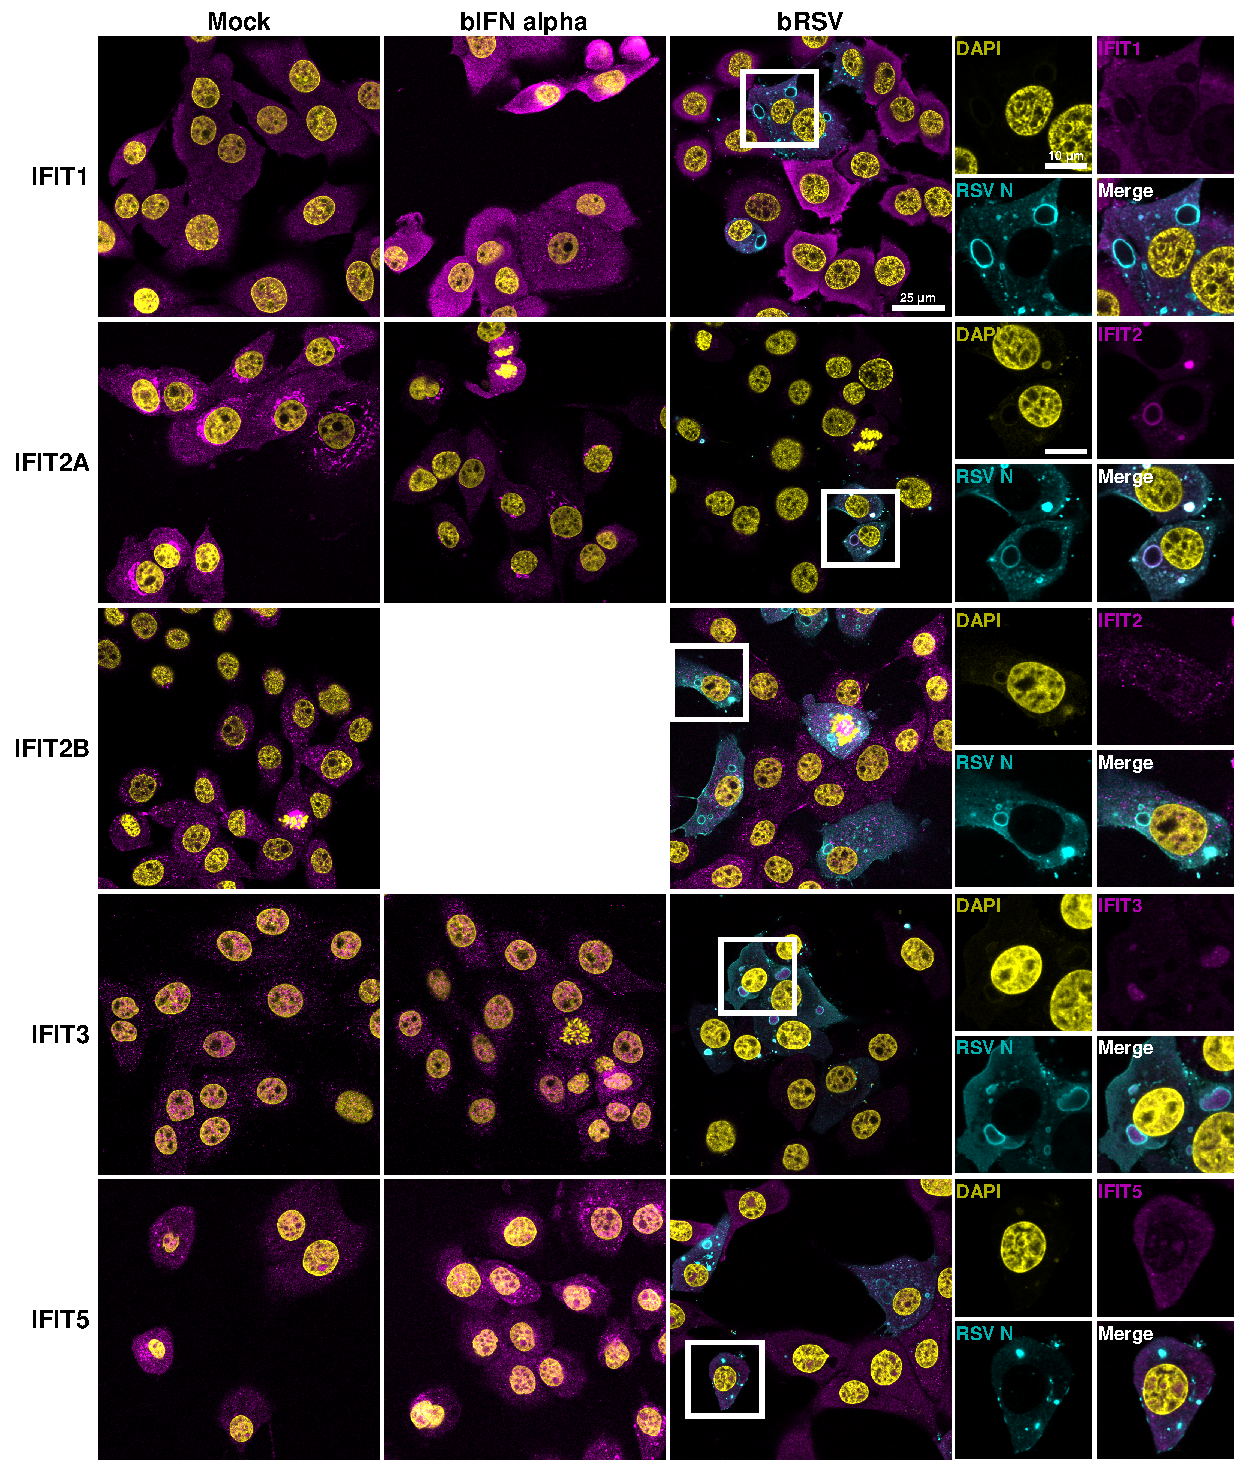
\includegraphics[width=1\linewidth]{09. Chapter 4/Figs/01. Localisation introduction/07. mdbk-merges-test.pdf}
    \caption[MDBK localisation mergers.]{MDBK localisation mergers. THIS IS A TEST TO SEE HOW IT WOULD LOOK!!!!!}
    \label{fig:MDBK localisation mergers}
\end{figure}


\begin{figure}
    \centering
    \includegraphics[width=1\linewidth]{09. Chapter 4/Figs/01. Localisation introduction/08. mdbk plots.png}
    \caption[MDBK localisation plots.]{MDBK localisation plots.}
    \label{fig:MDBK localisation plots}
\end{figure}
